\section{Generalities}
An effort has been made to keep the same notations between the mathematical framework and the \mudiff toolbox. Some explanations
(goal of the function and input/output arguments)
about a function \code{name_of_the_function} can be obtained by  typing the classical \matlab command window 
\begin{lstlisting}
help name_of_the_function;
\end{lstlisting}

Because \mudiff includes all the integral operators that are needed in scattering (traces and normal derivative
traces of the single- and double-layer potentials), a large class of scattering problems can be solved as long as the shape
of the obstacles is circular. 
Concerning the geometrical configurations, any deterministic or random distribution of disks is possible. Finally,
\mudiff includes post-processing facilities like e.g.: surface and far-fields computations, total and scattered exterior (near-field)
visualization\ldots

We now introduce the \mudiff  toolbox based on Matlab by explaining the main predefined functions and their relations
with the previous mathematical derivations. Section \ref{presentationnotation} gives a presentation and introduces the notations.
Section \ref{sec:PreProcessing}  shows how to define the scattering configuration (geometry and physical parameters). Section
 \ref{sec:ResolutionMuDiff}  presents the way the integral equations must be defined and solved.
  Finally, section \ref{sec:PostProcessing} describes the data post-processing. 

The \mudiff toolbox  is organized following the five subdirectories (see also Figure \ref{fig:arbo} for a diagram of the directory arborescence)
\begin{itemize}
\item \texttt{mudiff/PreProcessing/}: pre-processing data functions (incident wave and geometry) (section \ref{sec:PreProcessing}).
\item \texttt{mudiff/IntOperators/}: functions for the four basic integral operators (dense and sparse structure)
used in the definition of the integral equations to solve (section \ref{sec:ResolutionMuDiff}). 
\item \texttt{mudiff/PostProcessing/}: post-processing functions of the solution (trace and normal derivative traces,
computation of the scattered/total wavefield 
at some points of the spatial domain or on a grid, far-field and RCS) 
(section \ref{sec:PostProcessing}).
\item \texttt{mudiff/Common/}: this directory includes functions that are used in \mudiff but which does not need to be known
from the standard user point of view.
\item \texttt{mudiff/Examples/}: various scripts are presented for the user in standard configurations.
\item \texttt{mudiff/Solver/}: Module to solve the multiple scattering problem directly (the integral equation is build and solved automatically). See chapter \ref{chap:solver} for more information.
\end{itemize}
In addition, the \mudiff user guide, license and credits can be found under the directory \texttt{mudiff/Doc/}.


\begin{figure}[p]
\tikzstyle{every node}=[draw=black,thick,anchor=west]
\begin{tikzpicture}[%
  grow via three points={one child at (0.5,-0.7) and
  two children at (0.5,-0.7) and (0.5,-1.4)},
  edge from parent path={(\tikzparentnode.south) |- (\tikzchildnode.west)}]
  \node {mu-diff/}
    child { node {Common}}
    child { node {Doc}}
    child { node {Examples}
      child { node {Benchmark}}
      child { node {TimeReversal}
      	  child { node {FarField}
      	    child { node {Common}}
      	    child { node {NonPenetrable}}
      	    child { node {Penetrable}}
      }
    }
    }
    child [missing] {}
    child [missing] {}
    child [missing] {}
    child [missing] {}
    child [missing] {}
    child [missing] {}
    child { node {IntOperators}
      child{node{Dense}
         child{node{Interface}
         child{node{Block}}
         child{node{Full}}
         }
      }
          child [missing] {}
    child [missing] {}
    child [missing] {}
      child{node{Sparse}
        child{node {Functions}}
         child{node{Interface}
           child{node{Block}}
           child{node{Full}}
         }
      }
    }
    child [missing] {}
    child [missing] {}
    child [missing] {}
    child [missing] {}
    child [missing] {}
    child [missing] {}
    child [missing] {}
    child [missing] {}
    child [missing] {}
    child { node {PostProcessing}
      child { node {FarField}
        child { node {Interface}}
       }
       child [missing] {}
      child { node {Geometry}}
      child { node {IncidentWave}}
      child { node {NearField}
        child { node {Functions}}
        child { node {Interface}}
       }
      }
    child [missing] {}
    child [missing] {}
    child [missing] {}
    child [missing] {}
    child [missing] {}
    child [missing] {}
    child [missing] {}
    child { node {Preprocessing}
        child { node {Fourier}}
        child { node {Geometry}}
        child { node {IncidentWave}
           child { node {Full}}
           child { node {Block}}
         }
	}
;
\end{tikzpicture}
\caption{Arborescence of \mudiff toolbox.}
\label{fig:arbo}
\end{figure}

\section{Common argument and notations\label{presentationnotation}}

A large number of arguments of the \mudiff functions are similar. For the sake of conciseness and if nothing is specified, the following arguments refer to
 the ones given in the Tables below, where the indices $p$ and $q$ vary from $1$ to $M$ (or \code{N\_scat} in the \mudiff scripts). In addition, any
  function or value specific to \mudiff is written with the following \code{font}. 

\paragraph{Geometry}
\label{sec:geometry}

\begin{center}
%\rowcolors{1}{white}{gray}
\begin{tabular}{|c |c | p{10cm}|}
\hline Name & Size & Description\\[0.2cm]\hline\hline
\tabcode{N\_scat} & $[1\times 1]$ & number of obstacles $M$\\\hline
\tabcode{O} & $[2\times \Nscat]$ & matrix of the centers of the disks such that \code{O(1,p)} (resp. \code{O(2,p)}) is the abscissa (resp. ordinate) of the $p^{\textrm{th}}$ obstacle\\\hline
\tabcode{Op} & $[2\times 1]$ & coordinates of the $p^{\textrm{th}}$ scatterer\\\hline
\tabcode{Oq} & $[2\times 1]$ & coordinates of the $q^{\textrm{th}}$ scatterer\\\hline
\tabcode{a} & $[1\times \Nscat]$ & vector of the radii of the disks such that \code{a(p)} is the radius of the $p^{\textrm{th}}$ scatterer\\\hline
\tabcode{ap} & $[1\times 1]$ & radius of the $p^{\textrm{th}}$ scatterer\\\hline
\tabcode{aq} & $[1\times 1]$ & radius of the $q^{\textrm{th}}$ scatterer\\\hline
\end{tabular}
\end{center}

\newpage

\paragraph{Parameters (wavenumbers, incident waves, Fourier series expansions, \ldots)}
\begin{center}
\begin{tabular}{|c |c | p{10cm}|}
\hline Name & Size & Description\\[0.2cm]\hline\hline
\tabcode{beta\_inc} & $[1\times 1]$ & angle of direction $\beta$ of a plane wave $e^{ik (\cos(\beta)x_{1} + \sin(\beta)x_{2})}$\\\hline
\tabcode{XS} & $[2\times 1]$ & center $(x_{1s},x_{2s})$ of a point source: $x_{1s}=$\code{XS(1)} and $x_{2s}=$\code{XS(2)}. A point source wave is given by
 $$\frac{i}{4}\Hz(k\|\xx-\xx_s\|),$$ with $\xx=(x_{1},x_{2})$ and $\xx_s=(x_{1s},x_{2s})$, with $\Hz$ the zeroth order Hankel function of the first-kind\\\hline
\tabcode{k} & $[1\times 1]$ & wavenumber $k$ in the vacuum\\\hline
\tabcode{k\_int} & $[1\times \Nscat]$ & wavenumbers in the obstacles: $\kintp=$\code{k\_int(p)}. If \code{k\_int} is a scalar then $\kintp$ = \code{k\_int} for all $p=1,...,M$\\\hline
\tabcode{M\_modes} & $[1\times \Nscat]$ & vector of index of truncation of the Fourier series, \ie \code{M\_modes(p)}=$\Np$\\\hline
\tabcode{Np} & $[1\times 1]$ & corresponds to the truncation index $\Np$  in the Fourier series\\\hline
\tabcode{Nq} & $[1\times 1]$ & corresponds to the truncation index $\Nq$  in the Fourier series\\\hline
\end{tabular}
\end{center}

\paragraph{Integral operators (see chapter \ref{chap:math})}
\begin{center}
\begin{tabular}{|c |c | c || p{7cm}|}
\hline\multicolumn{3}{|c||}{\mudiff} & {\centering Mathematics} \\
 index  &  char or \{cell string\} & abbreviation &  \\\hline\hline
0  & 'Z' &- & null operator \\[0.2cm]\hline
1  &'I'& \tabcode{Identity} & identity\\[0.2cm]\hline
2  &'L'& \tabcode{SingleLayer} & $\dsp L\rho = \int_{\Gamma}G(\xx,\yy)\rho(\yy)\;\dd\yy$\\[0.2cm]\hline
3  &'M'& \tabcode{DoubleLayer} & $\dsp M\lambda = -\int_{\Gamma}\dny G(\xx,\yy)\lambda(\yy)\;\dd\yy$\\[0.2cm]\hline
4   &'N'& \tabcode{DnSingleLayer}& $\dsp N\rho = \dnx\int_{\Gamma}G(\xx,\yy)\rho(\yy)\;\dd\yy$\\[0.2cm]\hline
5   &'D'& \tabcode{DnDoubleLayer}&$\dsp D\lambda = -\dnx\int_{\Gamma}\dny G(\xx,\yy)\lambda(\yy)\;\dd\yy$\\[0.2cm] \hline
6 & 'P' or \{'Lprec'\} & \tabcode{PrecondDirichlet}& $\hat{L}^{-1}L$: single-scattering preconditioned trace of the single-layer operator (see \S\ref{sec:SingleScat})\\[0.2cm]\hline
7  & 'Q' or \{'Dprec'\} & \tabcode{PrecondNeumann}&  $\hat{D}^{-1}D$: single-scattering preconditioned normal derivative trace of the double-layer operator (see \S\ref{sec:SingleScat})\\ \hline
\end{tabular}
\end{center}


\section{Pre-processing}\label{sec:PreProcessing}

The pre-processing in \mudiff consists in defining the right-hand side (or the incident wave) and the geometry (the obstacles). The associated functions are located respectively in the folders \folder{mudiff/PreProcessing/IncidentWave} and in \folder{mudiff/PreProcessing/Geometry}.

\subsection{Geometry: creating the obstacles}
\label{sec:placementObstacles}

The obstacles are stored in memory as a row vector \code{a} containing the radii of the disks and a [$2\times\code{N\_scat}$] matrix \code{O} with the centers of the disks (\code{O(1,p}=$x$- and \code{O(2,p}=$y$- coordinates of the center of the $p^{th}$ disk). These two arrays can be created either manually or by
using some built-in functions.

\subsubsection{Manually}

The disks can be created manually by simply creating the two variables \code{O} and \code{a} containing respectively the coordinates of the disks and their radii. For example, for three obstacles placed at points $(-1,2)$, $(5,5)$ and $(-15,10)$ with respective radii $0.1$, $0.5$ and $10$, one gets
\begin{lstlisting}
O = [-1, 5, 2 ; -15, 5, 10];
a = [0.1, 0.5, 10];
\end{lstlisting}

\subsubsection{Periodic placement}
\label{secFun:RectangularLattice}
\label{secFun:TriangularLattice}

Two built-in functions are available with the toolbox to  periodically place some disks, with a rectangular or a triangular lattice, as shown on Figure \ref{fig:lattices}. The two functions must be called as follows, first for the rectangular lattice
\begin{lstlisting}
O = RectangularLattice(bx, by, Nx, Ny, OPTIONS);
\end{lstlisting}
and second for the triangular lattice
\begin{lstlisting}
O = TriangularLattice(bx, by, Nx, Ny, OPTIONS);
\end{lstlisting}
where the arguments are
\begin{itemize}
\item \code{bx}: distance separating two centers in the $x_{1}$-direction (be careful with the radii of the disks to avoid overlapping!).
\item \code{by}: distance separating two row of obstacles in the $x_{2}$-direction.
\item \code{Nx}: number of disks in a row.
\item \code{Ny}: number of rows.
\end{itemize}
For both functions, the vector of radii must be built separately and manually. For a set of unitary disks, the following command is used
\begin{lstlisting}
a = ones(size(O,2));
\end{lstlisting}

The available options are (same for \RectangularLattice and \TriangularLattice)
\begin{itemize}
\item \code{RectangularLattice(..., 'Origin', Ostart)}
places the first disk at \code{Ostart} position, \code{Ostart} being a [2x1] vector. (Default: $[0;0]$).
\item \code{RectangularLattice(..., 'Centered', Ocenter)}
center the collection on the point \code{Ocenter}, \code{Ocenter} being a [2x1] vector. (Default: none but replace Ostart value).
 \item \code{RectangularLattice(..., 'Direction', DIR)}
places the row in the increasing  (\code{DIR}�= +1) or decreasing $x_{2}$-direction (\code{DIR}�= -1). The default value is: \code{DIR} = +1.
\end{itemize}

\paragraph{Example:} Building a rectangular lattice of  $3 \times 4$ unit disks. Each disk is separated from the other by
  a distance equal to $1.5$ (so the centers are separated from a distance of $3.5$)
\begin{lstlisting}
O = RectangularLattice(3.5, 3.5, 3, 4);
a = ones(size(O,2));
\end{lstlisting}

\begin{figure}
\centering
\subfigure[Rectangular lattice]{\begin{tikzpicture}
 \pgftext{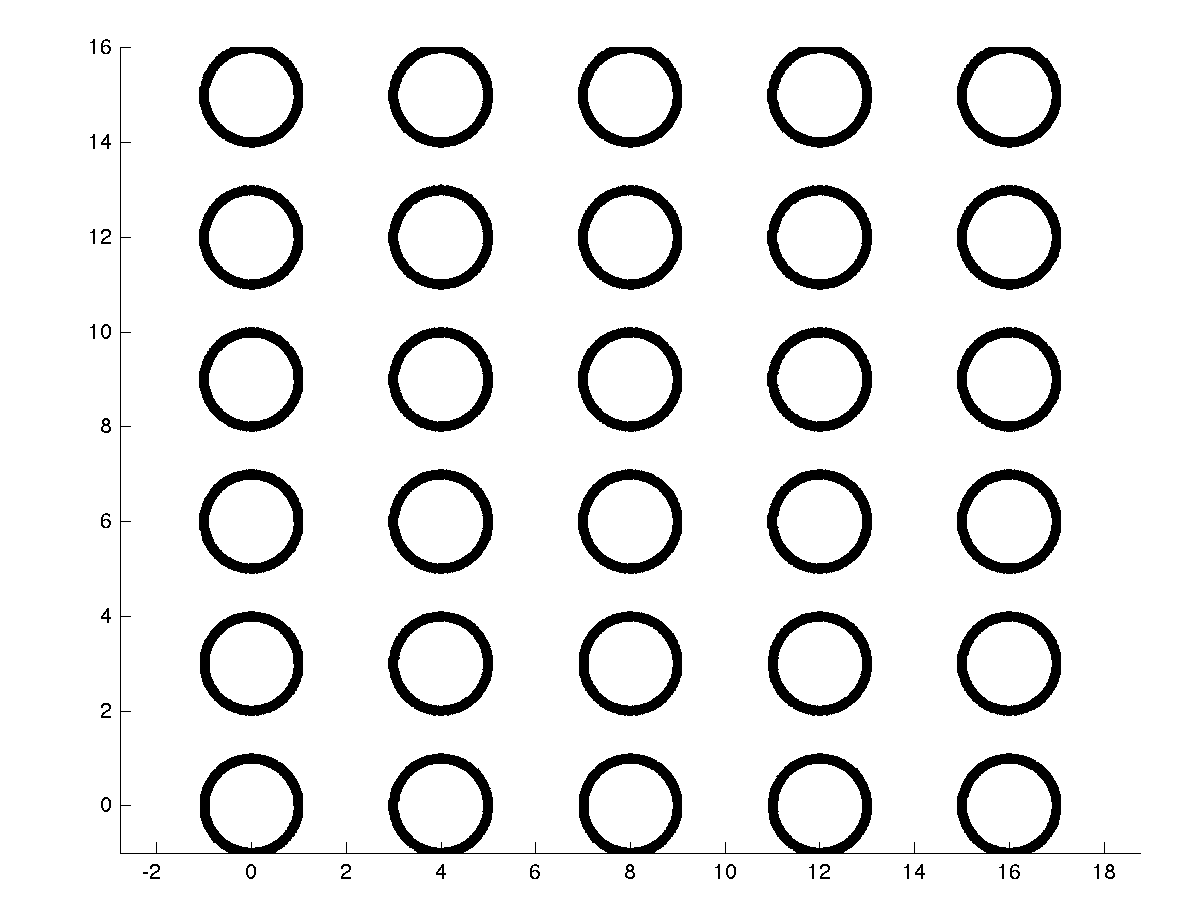
\includegraphics[width=0.45\textwidth]{./img/obstacles/rectangular.png}}
 \draw (10pt,-75pt) node[below]{\footnotesize $x_{1}$} ;
 \draw (-92pt,10pt) node[below]{\footnotesize $x_{2}$} ;
\end{tikzpicture}}\quad\subfigure[Triangular lattice]{\begin{tikzpicture}
 \pgftext{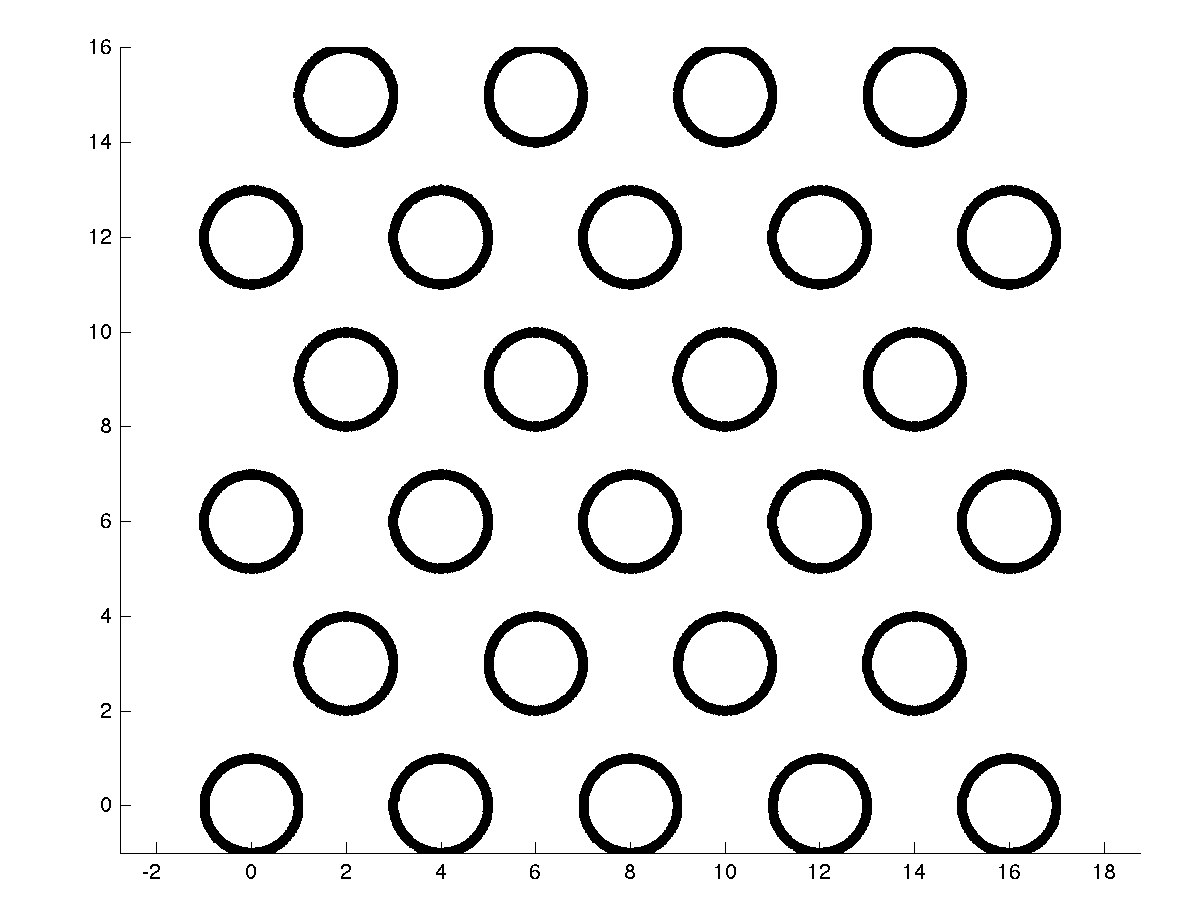
\includegraphics[width=0.45\textwidth]{./img/obstacles/triangular.png}}
 \draw (10pt,-75pt) node[below]{\footnotesize $x_{1}$} ;
 \draw (-92pt,10pt) node[below]{\footnotesize $x_{2}$} ;
\end{tikzpicture}}
\caption{Rectangular (left) and triangular (right) lattice with \code{bx} = 3, \code{by} = 4, \code{Nx} = 5, \code{Ny}=6.}
\label{fig:lattices}
\end{figure}


\subsubsection{Random placement}
\label{secFun:CreateRandomDisks}

The toolbox \mudiff provides a function \CreateRandomDisks to randomly place \code{N\_scat} obstacles in a box $[\code{xmin}, \code{xmax}]\times[\code{ymin},\code{ymax}]$ with a random radius. In its simplest version, the function is called as
\begin{lstlisting}
[O, a] = CreateRandomDisks(xmin, xmax, ymin, ymax, N_scat);
\end{lstlisting}
In that case, \CreateRandomDisks builds \code{N\_scat} disks with unit radius in the  box. The function takes care to not overlap the disks. Note that it is possible that the function does not succeed to place the obstacles (e.g. if the user specifies  too many obstacles in a box which is not large enough). This is the reason why 
 a security test has been set: only $500$ possible placements are allowed per disk. 

The function comes along with a large set of optional arguments
\begin{lstlisting}
[O, a] = CreateRandomDisks(xmin, xmax, ymin, ymax, N_scat, 
           amin, amax, dmim, dmax, O_avoid, a_avoid, dmin_avoid, dmax_avoid);
\end{lstlisting}
where each additional argument is optional (but the order must be kept (\code{amin} must be set, then \code{amax}, etc...!) and given by
\begin{center}
\begin{tabular}{|c |c|c | p{10cm}|}
\hline Variable & Type & Default & Description\\\hline
\tabcode{amin} & scalar  & 1 & minimal (random) radius of the obstacles allowed \\\hline
\tabcode{amax} & scalar  & 1 & maximal (random) radius of the obstacles  allowed\\\hline
\tabcode{dmin} & scalar & \tabcode{realmin} & minimal distance allowed between two obstacles (not between the centers!). Setting $\leq 0$  value will set \code{dmin} to \code{realmin} (\ie ignore it)\\\hline
\tabcode{dmax} & scalar & \tabcode{realmax} & maximal distance allowed between two obstacles (not between the centers!). The maximal distance is efficiently reached! Setting $\leq 0$  value will set \code{dmax} to \code{realmax} (i.e. ignore it)\\\hline
\tabcode{O\_avoid} & $[2 \times N]$ & \tabcode{[]} & center of \code{N} hole(s) where the obstacles must not overlap. Useful for example for the points source location\\\hline
\tabcode{a\_avoid} & $[1 \times N]$ & \tabcode{[]} & radii of the \code{N} holes\\\hline
\tabcode{dmin\_avoid} & $[1 \times N]$ & \tabcode{[]} & minimal distance between an obstacle and a hole\\\hline
\end{tabular}
\end{center}
The ``holes'', represented by the \code{*\_avoid} arguments, are circular regions where the obstacles must not overlap, for example where a point source is emitting a wave. 

\paragraph{Example 1:} creating \code{N\_scat} random disks with random radii is realized by the command
\begin{lstlisting}
[O, a] = CreateRandomDisks(xmin, xmax, ymin, ymax, N_scat, amin, amax);
\end{lstlisting}
\paragraph{Example 2:} building 7 obstacles in the box $[-10,10]\times[-10,10]$ with radii between $0.1$ and $0.5$. The disks must be separated 
 by a minimal distance equal to $0.1$ and without maximal value. The command is then
\begin{lstlisting}
[O, a] = CreateRandomDisks(-10, 10, -10, 10, 7, 0.1, 0.5, 0.1, -1);
\end{lstlisting}
\paragraph{Example 3:} now consider that a point source is located at $(2,2)$ and that the obstacles must be separated from the source by at least a distance 
equal to $0.3$. Then, the ``\code{*\_avoid}'' arguments can be used and the resulting function call is
\begin{lstlisting}
[O, a] = CreateRandomDisks(-10, 10, -10, 10, 7, 0.1, 0.5, 0.1, -1, [2;2], 0.3);
\end{lstlisting}
The disk centered at $(2,2)$ with radius $0.3$ is then avoided. A second option
 is to set \code{a\_void} to zero and set the minimal distance \code{dmin\_avoid} to $0.3$
\begin{lstlisting}
[O, a] = CreateRandomDisks(-10, 10, -10, 10, 7, 0.1, 0.5, 0.1, -1, [2;2], 0, 0.3);
\end{lstlisting}


\begin{remark}
\label{secFun:CheckPlacement}
To check if a disk is correctly placed, \CreateRandomDisks calls the \CheckPlacement function which can also be useful for a user who is placing the obstacles manually.
\end{remark}

\subsubsection{Removing disks}
\label{secFun:RemoveDisk}

The function \RemoveDisk aims to remove some disks of the geometrical configuration, either disk by disk, by row, by column or by radius. This can be useful for example to delete a row of disks. Here is the syntax
\begin{lstlisting}
[O,a] = RemoveDisk(O_old, a_old, ...);
\end{lstlisting}
where \code{O\_old} and \code{a\_old} are the centers and radii of the current geometry. Without optional argument, the function has no effect. The available arguments are
\begin{itemize}
\item \code{[O,a] = RemoveDisk(..., 'X', [X1, X2, .., XN]);}\\
Remove all the disks with a center which has an abscissa equal to \code{X1}, \code{X2}, \ldots, or \code{XN}.
\item \code{[O,a] = RemoveDisk(...,  'Y', [Y1, Y2, ..., YN]);}\\
Remove all the disks with a center which has an ordinate equal to \code{Y1}, \code{Y2}, \ldots, or \code{YN}.
\item \code{[O,a] = RemoveDisk(..., 'XY', [[X1;Y1], [X2;Y2], ..., [XN;YN]]);}\\
Remove all the disks with a center with coordinates \code{[X1;Y1]}, \code{[X2;Y2]}, \ldots, or \code{[XN;YN]}.
\item \code{[O,a] = RemoveDisk(..., 'Radius', [a1, a2, ..., aN]);}\\
Remove all the disks with a radius equal to \code{a1}, \code{a2}, \ldots, or \code{aN}.
\item \code{[O,a] = RemoveDisk(..., 'Verbosity', VERBOSITY);}\\
set \code{VERBOSITY} to 0 to avoid display message, to 1 to only show results, and to $>1$ to see everything (default).
\item \code{[O,a] = RemoveDisk(..., 'Tol', TOL);}\\
Tolerance used for the conditional statement (default $10^{-10}$).
\end{itemize}

\paragraph{Example 1:} Remove all the obstacles that are either on the row of with abscissa equal to $1$ or on the column with an ordinate equal to $2.5$
\begin{lstlisting}
[O,a] = RemoveDisk(O_old, a_old, 'X', 1, 'Y', 2.5);
\end{lstlisting}
\paragraph{Example 2:} Remove the obstacles centered at $(2,5)$ and $(3,4)$
\begin{lstlisting}
[O,a] = RemoveDisk(O_old, a_old, 'XY', [2, 3; 5, 4]);
\end{lstlisting}
\paragraph{Example 3:} Create a periodic placement of $11 \times 11$ unit disks, separated by a distance equal to $1$, then remove the
 middle line and the middle column, as shown on Figure \ref{fig:removeDisks}. The central disk is moreover centered at $(0,0)$.
\begin{lstlisting}
bx = 3; by = 3;
Nx = 11; Ny = 11;
O = RectangularLattice(bx, by, Nx, Ny, 'Centered', [0,0]);
a = ones(1, size(O, 2));
[O, a] = RemoveDisk(O, a, 'X', 0, 'Y', 0);
\end{lstlisting}

\begin{figure}[h!]
\centering
\begin{tikzpicture}
 \pgftext{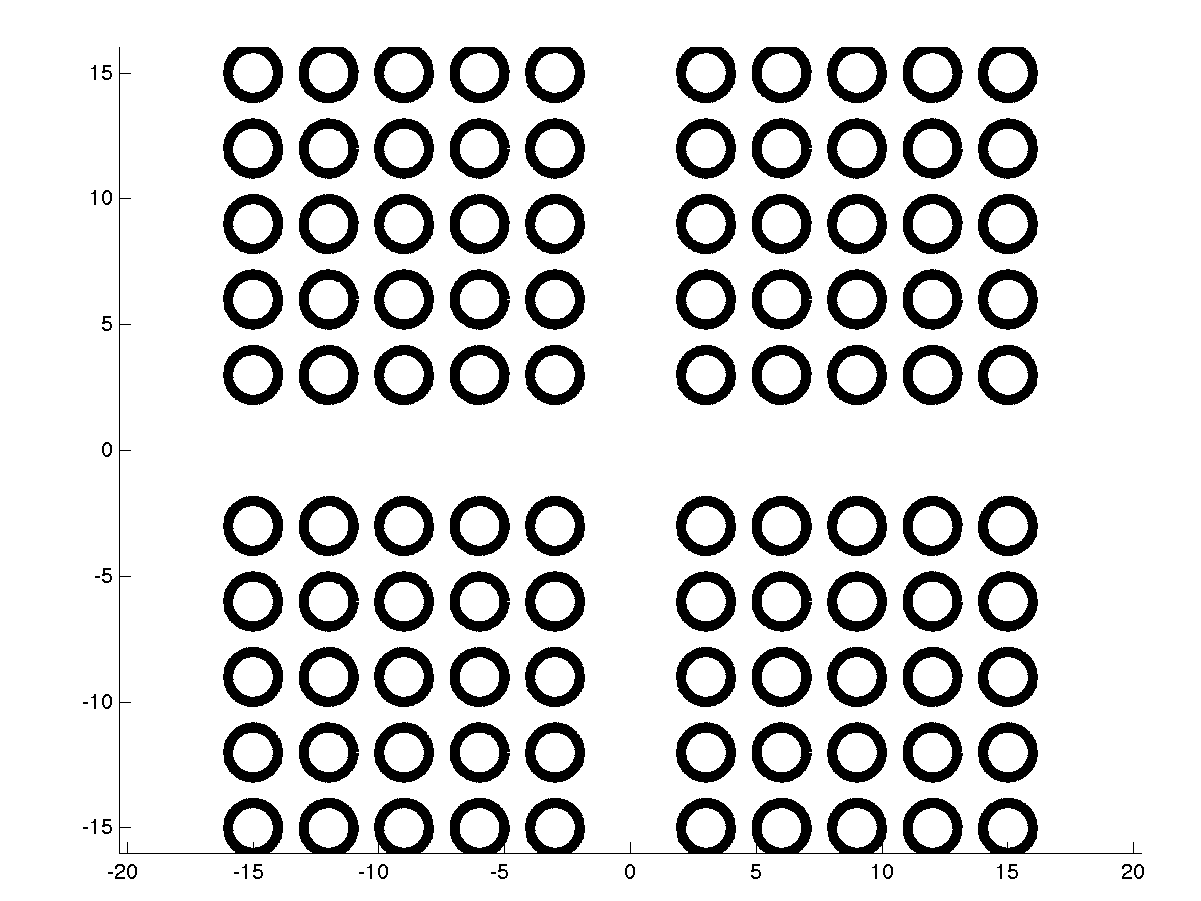
\includegraphics[width=0.45\textwidth]{./img/obstacles/removeDisks.png}}
 \draw (10pt,-75pt) node[below]{\footnotesize $x_{1}$} ;
 \draw (-92pt,10pt) node[below]{\footnotesize $x_{2}$} ;
\end{tikzpicture}
\caption{Periodic placement with a row and a column deleted.}
\label{fig:removeDisks}
\end{figure}



\subsection{Truncation of the Fourier series}
\label{secFun:FourierTruncation}

To help the user, the formula (\ref{eqEqInt:CFIEDapp}) has been coded in \mudiff. The values of $\Np$ are stored in a Matlab vector of size $[1\times\code{N\_scat}]$ called \code{M\_modes} in \mudiff. Computing \code{M\_modes} only involves the radii of the disks and the wavenumber \code{k}, which is assumed to be created by the user
\begin{lstlisting}
M_modes = FourierTruncation(a, k);
\end{lstlisting}
The resulting vector is such that \code{M\_modes(p)}=$\Np$, where $\Np$ satisfies (\ref{eqEqInt:CFIEDapp}), with obviously a minimal value equal to
 $0$ (which consists in only one mode). If \code{k} is a vector (which corresponds to one wavenumber per obstacle), then
  \FourierTruncation uses formula (\ref{eqEqInt:CFIEDapp})  with \code{k(p)} as the wavenumber.
The following options are moreover available
\begin{itemize}
\item \code{M\_modes = FourierTruncation(..., 'Min', MIN);}\\
To force a minimal value: \code{M\_modes(p)} is then either the min value between \code{MIN} and formula (\ref{eqEqInt:CFIEDapp}). 
\item\code{M\_modes = FourierTruncation(..., 'Tol', TOL);}\\
The tolerance, set by default to $10^{-10}$, is then set to \code{TOL}.
\end{itemize}

\subsection{Incident waves}

\subsubsection{Generalities}
\label{secFun:PlaneWave}
\label{secFun:DnPlaneWave}
\label{secFun:PointSource}
\label{secFun:DnPointSource}
\label{secFun:PlaneWavePrecond}
\label{secFun:DnPlaneWavePrecond}
\label{secFun:BlockPlaneWave}
\label{secFun:BlockDnPlaneWave}
\label{secFun:BlockPointSource}
\label{secFun:BlockDnPointSource}
\label{secFun:BlockPlaneWavePrecond}
\label{secFun:BlockDnPlaneWavePrecond}

Two different incident waves are available in the \mudiff toolbox: the plane wave and the point source wave. The user can build his
 own incident wave. They are all located in the directory \folder{PreProcessing/IncidentWave/}.

As explained in section \ref{secEqInt:SecondMembre}, a right-hand side $b$ is decomposed by blocks, each of these blocks representing one obstacle: $b= (b_p)_{p=1,\ldots,\Nscat}$. A different condition can be applied on two different obstacles (e.g. Dirichlet on $\Omega_1$ and Neumann on $\Omega_2$) or a different integral equation can be considered on each obstacle (e.g. EFIE on $\Omega_1$ and MFIE on $\Omega_2$). To this end, \mudiff builds each block separately thanks to the
function \BlockIncidentWave which computes the vector $b_p$. According to the input data, the function builds
 one of the available right-hand sides described in Table \ref{table:Uinc}.

On the other hand, the common function \IncidentWave computes the whole vector $b$. For all obstacles $p$, the function
 \BlockIncidentWave is called and the whole vector is assembled. 

In addition, for all the incident waves, an interface function is available. These easy-to-use interfaces build
 the whole vector on only one pattern (trace of plane wave, normal derivative of a point source wave, \ldots). 
  They are located in the \folder{interface/} directory and their names allow an easy interpretation
   (see also table \ref{table:Uinc}, column \mudiff name): \PlaneWave, \PointSource, \DnPlaneWave,\ldots. Let us recall that the help informations
    of the interface functions contains the mathematical description of the incident wave.

The two main functions, \BlockIncidentWave and \IncidentWave, are now detailed.

\subsubsection{\code{BlockIncidentWave}}
\label{secFun:BlockIncidentWave}

This function computes the block vector of \textbf{the opposite of} the coefficients of an incident wave, either the trace of the normal derivative trace, on one of the obstacles, in the Fourier bases. Its syntax is
\begin{lstlisting}
Bp = BlockIncidentWave(Op, ap, Np, k, TypeOfWave, Param);
\end{lstlisting}
where \code{TypeOfWave} is a scalar value specifying the incident wave (see table \ref{table:Uinc}) and \code{Param} is the parameter of the wave: angle of direction, position of a point source, \ldots. The returned value \code{Bp} is a column vector of length $2\code{Np}+1$.
\begin{table}
\begin{tabular}{|c| c |c| p{9cm}| }
\hline Value & \mudiff function name & Param & Description\\\hline
1 & \code{PlaneWave} & \code{beta\_inc} & trace of a plane wave of angle of direction \code{beta\_inc}. A plane wave is defined by $e^{ik(\cos(\beta)x_{1}
 + \sin(\beta)x_{2}}$\\\hline
2 & \code{DnPlaneWave} & \code{beta\_inc} & normal derivative of a plane wave of angle of incidence \code{beta\_inc}\\\hline
3 & \code{PointSource} & \code{XS} & trace of the wave emitted by a point source placed at \code{XS}. Such a wave is defined in \mudiff by 
$$\frac{i}{4}\Hz(k\|\xx-\xx_s\|)$$ \\\hline
4 & \code{DnPointSource} & \code{XS} & normal derivative  trace of the wave emitted by a point source placed at \code{XS}\\\hline
5 & \code{PlaneWavePrecond} & \code{beta\_inc} & same as \code{PlaneWave} but multiplied by the inverse of  the single-layer block diagonal operator (see
 section \ref{preconDiskTheory} on the single-scattering preconditioner) \\\hline
6 & \code{DnPlaneWavePrecond} & \code{beta\_inc} & same as \code{DnPlaneWave} but multiplied by the inverse of the double-layer block diagonal  operator \\\hline
\end{tabular}
\caption{Right-hand sides already coded in $\mu$-diff.}
\label{table:Uinc}
\end{table}

\subsubsection{\code{IncidentWave}}
\label{secFun:IncidentWave}
The function call is the following
\begin{lstlisting}
B = IncidentWave(O, a, M_modes, k, TypeOfWave, Param)
\end{lstlisting}
The resulting vector \code{B} is of size $\sum_{p=1}^{\Nscat}(2\code{M\_modes}(p)+1)$. The value \code{Param} is the same as for \BlockIncidentWave whereas \code{TypeOfWave} is a vector of size $\Nscat$, where \code{TypeOfWave}(p) is the fixed choice for the block $b_p$. In other word, the block $b_p$ is built by calling
the function with the arguments \code{BlockIncidentWave(Op, ap, Np, k, TypeOfWave, Param);}. To simplify, if \code{TypeOfWave} is a scalar value, then it is considered as a vector with the same scalar value.

\paragraph{Example 1:} Building a vector associated to the trace of an incident plane wave of direction \code{beta\_inc} is done thanks to the following command (the ``$1$ argument'' refers to as \code{PlaneWave})
\begin{lstlisting}
B = IncidentWave(O, a, M_modes, k,  1, beta_inc);
\end{lstlisting}
or by using the interface function
\begin{lstlisting}
B = PlaneWave(O, a, M_modes, k, beta_inc);
\end{lstlisting}
\paragraph{Example 2:} For two obstacles and a point source centered at $(1,2)$, if $b_1$ is the trace of the wave and $b_2$ is the normal derivative trace, then
\begin{lstlisting}
B = IncidentWave(O, a, M_modes, k,  [3;4],[1;2]);
\end{lstlisting}
In other words, this builds the vector (\code{[3,4]} can be translated as \code{PointSource, DnPointSource})
$$
b = \left(\begin{array}{c}
-\uinc|_{\Gamma_1}\\
-\dn\uinc|_{\Gamma_2}\\
\end{array}\right),
$$
where $$\uinc = \frac{i}{4}\Hz(k\|\xx-\xx_s\|),$$ with $\xx_s = [1,2]$.
\begin{remark}
Remember that the resulting vector corresponds to the opposite of the trace or normal derivative trace!
\end{remark}


\section{Integral operators}
\label{sec:ResolutionMuDiff}

\subsection{Generalities}

The functions defining the integral operators are available in the directory \folder{IntOperators/} which has the \folder{Dense/}
and \folder{Sparse/} subdirectories for the dense (matrix) and sparse (@function) representations of the four basic integral operators used in scattering,
i.e. $\Lb$, $\Mb$, $\Nb$ and $\Db$, given in their infinite dimensional operator versions by respectively (\ref{eq:InfL}), (\ref{eq:InfM}), (\ref{eq:InfN}) and (\ref{eq:InfD}). Preconditioned versions of the operators by their single-scattering operators \cite{Thi14} are also defined. Following Proposition \ref{prop:SingleScat}, only $\widehat{L}^{-1}L$ (EFIE Dirichlet) and $\widehat{D}^{-1}D$ (EFIE Neumann) are provided since they are the only ones needed for the Dirichlet and Neumann problems. %These operators have moreover an analytic expression of every of their coefficients (see equations (\ref{eq:LL}) and (\ref{eq:DD}), in the infinite matrices case).

Two different types of storage can be used  within the \mudiff toolbox: dense and sparse. The assembly of the matrix is almost the same
 in both cases. The way \mudiff is developed is close to the mathematics for the assembly process, in the sense that the matrix $\Ab$ of an integral operator is built block-by-block ($\Abpq$). For both storages, two main functions exist: a ''block'' function (\BlockIntegralOperator and \SpBlockIntegralOperator) and a global matrix function (\IntegralOperator and \SpIntegralOperator) which assemble all the blocks into a matrix. This separation allows the user
 to either build a ''simple'' matrix for one operator or to construct a more ''complex'' matrix where each block represents a different operator or a linear combination of them. Let us also note  that all the operators have interface functions (located in \folder{Dense/Interface} or \folder{Sparse/Interface} folders). For example, \SingleLayer is the interface function of \IntegralOperator to build the single-layer operator, and \BlockSingleLayer the one for
  \BlockIntegralOperator. The same applies for the sparse storage with a prefix \code{Sp}:  \SpSingleLayer,  \SpBlockSingleLayer.


The dense storage should be preferred for solving small scale problems (most particularly low frequency problems), when the memory storage and the CPU
 cost is not a problem, where the sparse storage must be used when the limits are reached. For the sparse storage, which is detailed later, the block
  matrices are stored through vectors and the matrix-vector product is then fast when an iterative Krylov subspace solver is used.
This is essentially a suitable strategy  when a sufficiently high number of modes $N_{p}$ is required per obstacle, i.e. for large enough wave numbers $k$.
  The drawback is that some instabilities may arise in the numerical process
   if the truncations of the Fourier series are not done correctly. The formula (\ref{eqEqInt:CFIEDapp}) provides
   a stable result following \cite{AntChnRam08}.



%Two different type of storage are provided with the \mudiff toolbox: dense and sparse. The dense storage the whole matrix in memory whereas the sparse version uses the special structure of the matrix of an integral operator to store it. The sparse storage in \mudiff and this user guide has nothing to deal with the sparse storage provided in \matlab such as \texttt{sparse} function. The dense storage is easier to use and works pretty well for small scale problems. It also presents the advantage of providing the whole matrix of the integral operator, which can be useful for spectrum analysis for example. On the other hand, for a large number of circular obstacles and/or for large frequency, the memory storage becomes too important and the sparse version must be used. One should be however careful: the sparse matrix-vector product, based on the cross-correlation (\texttt{xcorr} \matlab function), is very sensitive to the number of modes chosen in the truncation of the Fourier series. Indeed, if too many modes are kept, the matrix-vector product show to be unstable. The formula (\ref{eqEqInt:CFIEDapp}) seems to provide stability.
%
%To explain how the code works, let us take an example of one of the four boundary integral operator $L,M,N$ or $D$ being discretized as a generic matrix $\Ab = (\Abpq)_{1\leq p,q\leq \Nscat}$. Let us highlight that \mudiff can manage more complexe matrices, where two different blocks are not the discretization of the same operators or can even be a linear combination of operators. Nevertheless, if $\Ap$ is one of the four boundary integral operators, then as highlighted in previous chapter, $\Ab$ has the following structure, for $p,q=1,\ldots,\Nscat$ and $p\neq q$:
%\begin{itemize}
%\item $\Abpp$ is diagonal.
%\item $\Abpq$ is full and can be divided as $\Abpq = \AbpqL\Tbpq\AbpqR$ where $\AbpqL$ and $\AbpqR$ are diagonal and called respectively the left and right part, and $\Tbpq = (\Tbpqmn))$, with $\Tbpqmn = i\pi e^{??}H_0^{(1)}(k\bpq)$, is a Toeplitz matrix.
%\end{itemize}
%In the sparse version, diagonal submatrices $\Abpp,\AbpqL$ and $\AbpqR$  are stored as a vector of size respectively $2\Np+1$, $2\Np+1$ and $2\Nq+1$, and the Toeplitz matrices $\Tbpq$ are stored as vectors of size $2\Np+2\Nq-1$.
%
%This section is naturally divided in two part, the first being devoted to the dense storage and the second to the sparse version. The assembly, the storage and the usage of the matrices being significantly different.

\subsection{Available integral operators and numbering}
\label{seccode:IntOp}
\label{secFun:BlockSingleLayer}
\label{secFun:BlockDnSingleLayer}
\label{secFun:BlockDoubleLayer}
\label{secFun:BlockDnDoubleLayer}
\label{secFun:BlockPrecondDirichlet}
\label{secFun:BlockPrecondNeumann}
%\label{secFun:BlockCalderonProjector}
\label{secFun:BlockIdentity}
\label{secFun:SingleLayer}
\label{secFun:DnSingleLayer}
\label{secFun:DoubleLayer}
\label{secFun:DnDoubleLayer}
\label{secFun:PrecondDirichlet}
\label{secFun:PrecondNeumann}
%\label{secFun:CalderonProjector}
\label{secFun:Identity}

As for the incident wave, for each operator, there exists a function that builds the whole operator for the multiple scattering problem, both for the
 dense and sparse storages. The available operators are listed in Table \ref{table:IntOp}, with their unique identifier (integer), their unique char representation and string (if needed), their associated  name in \mudiff (useful to get their interface functions) and their definitions. It is more readable and convenient to use either the char or the string representation than the scalar one. 

\begin{table}
\begin{center}\begin{tabular}{|c| c|c| c|c|}
\hline Int. Op. & Id & Char or \{String\}& Function & Definition for $\xx\in\Gamma$\\\hline\hline
- & 0 & 'Z'&- & zero operator (null matrix)\\\hline
$I$ & 1& 'I' & \tabcode{Identity} & identity\\\hline
$L$ & 2 & 'L'& \tabcode{SingleLayer} & $\dsp L\rho(\xx) = \int_{\Gamma} G(\xx,\yy) \rho(\yy)\dd\yy$\\[0.25cm]\hline
$M$ & 3 & 'M'& \tabcode{DoubleLayer} & $\dsp M\lambda(\xx) = -\int_{\Gamma} \dny G(\xx,\yy) \lambda(\yy)\dd\yy$\\[0.25cm]\hline
$N$ & 4 & 'N'& \tabcode{DnSingleLayer} & $\dsp N\rho(\xx) = \dnx\int_{\Gamma} G(\xx,\yy) \rho(\yy)\dd\yy$\\[0.25cm]\hline
$D$ & 5 & 'D'& \tabcode{DnDoubleLayer} & $\dsp D\lambda(\xx) = -\dnx\int_{\Gamma} \dny G(\xx,\yy) \lambda(\yy)\dd\yy$\\[0.25cm]\hline
$\hat{L}^{-1}L$ & 6 & 'P' or \{'Lprec'\}& \tabcode{PrecondDirichlet} & single-layer preconditioned by its diagonal\\[0.25cm]\hline
$\hat{D}^{-1}D$& 7 & 'Q'or \{'Dprec'\}& \tabcode{PrecondNeumann} & double-layer preconditioned by its diagonal\\[0.25cm]\hline
\end{tabular}\end{center}
\caption{Available integral operators in $\mu$-diff, their (unique) identifier, char name and string name (for cell array), function name (interface) and the mathematical definition. 
The zero operator function does not have an interface function and the sparse version is obtained by adding the prefix
 \code{Sp} (\SpSingleLayer, \SpDnDoubleLayer,\ldots). The block interface functions are also prefixed by ''\code{Block}'' (\SpBlockSingleLayer, \BlockSingleLayer,\ldots).}
\label{table:IntOp}
\end{table}


\subsection{Dense storage}
\subsubsection{Building a block $\Abpq$}
\label{secFun:BlockIntegralOperator}

An elementary block matrix in a global matrix can be created by using the following function \BlockIntegralOperator
\begin{lstlisting}
Apq = BlockIntegralOperator(Op, ap, Np, Oq, aq, Nq, k, TypeOfOperator, Weight);
\end{lstlisting}
The \code{Weight} argument is optional and set to $1$ by default. The quantity \code{TypeOfOperator} specifies the integral operator to compute, thanks to the numbering of Table \ref{table:IntOp}. If \code{TypeOfOperator} is a unique value (scalar (e.g. =\code{2}), char (e.g. \code{'L'})), then the resulting matrix \code{Apq} is the elementary
matrix of the associated operator (e.g. $\Lbpq$). If \code{TypeOfOperator} is a row (e.g. \code{[1,3]}, \code{['I', 'M']} or cell \code{\{'I', 'M'\}}),  the sum of the
two operators is computed (e.g. $\Ibpq+\Mbpq$). Finally, the \code{Weight} quantity (of the same size as \code{TypeOfOperator})
 is the constant that is used to multiply the block and hence
$$
\Abpq = \sum_{\ell=1}^{N}\code{Weight}(\ell).\code{Operator}(\ell)
$$
where \code{Operator}$(\ell)$ is one of the integral operators.

\begin{remark}
The difference between the char and the string is purely computational: the char can be stored in an array or a cell whereas the string must be stored in a cell (due to possibly different size). The string representation only changes for $\hat{L}L$ and $\hat{D}D$, which can be written as respectively \code{'Lprec'} and \code{'Dprec'}. If a user wants to use \code{'Dprec'} instead of \code{'Q'}, (s)he must enclosed it into a cell \{\ldots\} instead of an array [\ldots]. The translation from char to scalar is done through the \Parser function. That's all (see example below).
\end{remark}

\begin{remark}
As the char or string representation is way more readable than the scalar one, in the next sections, examples will be based on this representation.
\end{remark}

\paragraph{Example 1:} Build the single-layer block $\Lbpq$
\begin{lstlisting}
%scalar representation
Apq = BlockIntegralOperator(Op, ap, Np, Oq, aq, Nq, k, 1);
%char representation
Apq = BlockIntegralOperator(Op, ap, Np, Oq, aq, Nq, k, 'L');
%string representation (cell array)
Apq = BlockIntegralOperator(Op, ap, Np, Oq, aq, Nq, k, {'L'});
\end{lstlisting}
\paragraph{Example 2:} Build the block $(\hat{\Lb}^{-1}\Lb)_{p,q}$
\begin{lstlisting}
%scalar representation
Apq = BlockIntegralOperator(Op, ap, Np, Oq, aq, Nq, k, 6);
%char representation
Apq = BlockIntegralOperator(Op, ap, Np, Oq, aq, Nq, k, 'P');
%string representation (cell array)
Apq = BlockIntegralOperator(Op, ap, Np, Oq, aq, Nq, k, {'Lprec'});
\end{lstlisting}
\paragraph{Example 3:} Build the block $0.5\times \Ibpq + \Nbpq$, appearing in the MFIE (\ref{eq:MFIE})
\begin{lstlisting}
%scalar representation
Apq = BlockIntegralOperator(Op, ap, Np, Oq, aq, Nq, k, [1, 4], [0.5, 1]);
%char representation
Apq = BlockIntegralOperator(Op, ap, Np, Oq, aq, Nq, k, ['I', 'N'], [0.5, 1]);
%string representation (cell array)
Apq = BlockIntegralOperator(Op, ap, Np, Oq, aq, Nq, k, {'I', 'N'}, [0.5, 1]);
\end{lstlisting}
\paragraph{Example 4:} Compute the sum of the four blocks: $0.5\times \Lbpq + 1.5 \times  \Mbpq + 2.5 \times  \Nbpq + 3.5 \times  \Dbpq$. \\
\begin{lstlisting}
%scalar representation
Apq = BlockIntegralOperator(Op, ap, Np, Oq, aq, Nq, k, [2, 3, 4, 5], 
                         [0.5, 1.5, 2.5, 3.5]);
%char representation
Apq = BlockIntegralOperator(Op, ap, Np, Oq, aq, Nq, k, ['L', 'M', 'N', 'D'], 
                         [0.5, 1.5, 2.5, 3.5]);
%string representation (cell array)
Apq = BlockIntegralOperator(Op, ap, Np, Oq, aq, Nq, k, {'L', 'M', 'N', 'D'}, 
                         [0.5, 1.5, 2.5, 3.5]);
\end{lstlisting}


\subsubsection{Assembling the matrix $\Ab$}
\label{secFun:IntegralOperator}

Now that the construction of an elementary block matrix is well-understood, building a global matrix is  easy thanks to the common function
\begin{lstlisting}
A = IntegralOperator(O, a, M_modes, k, TypeOfOperator, Weight);
\end{lstlisting}
As for \BlockIntegralOperator, the quantity \code{Weight} is optional and set to $1$ by default. Roughly speaking, \IntegralOperator  creates
a loop on all the obstacles $p$ and $q$, launches the following command
\begin{lstlisting}
Apq = BlockIntegralOperator(O(:,p), a(p), M_modes(p), O(:,q), a(q), M_modes(q), 
                                                    k, Tpq, Wpq);
\end{lstlisting}
and places \code{Apq} in the expected elementary block matrix of the global matrix. The quantities \code{Tpq} and \code{Wpq} are given by \code{TypeOfOperator} and \code{Weight} such that (\code{Weight} is of the same size as \code{TypeOfOperator} and so \code{Wpq} follows the same rules as \code{Tpq})
\begin{itemize}
\item If \code{TypeOfOperator} is one value then \code{Tpq} = \code{TypeOfOperator}. 
\item If \code{TypeOfOperator} is a row or a column vector then \code{Tpq} is an array given by \code{Tpq} = \code{TypeOfOperator}. 
\item If \code{TypeOfOperator} is a matrix then \code{Tpq} = \code{TypeOfOperator(p,q)}. 
\item If \code{TypeOfOperator} is a three-dimensional array, then \code{Tpq} is an array  given by \code{Tpq(:)} = \code{TypeOfOperator(p,q,:)}. 
\end{itemize}
%
%For example, this matrix will give,
%$$
%\left(\begin{array}{c c}
%2& 3\\
%4&5
%\end{array}\right)
%\longrightarrow
%\left(\begin{array}{c c}
%L^{1,1}& M^{2,1}\\
%N^{1,2} & D^{2,2}
%\end{array}\right)
%$$


\paragraph{Example 1:} The single-layer potential $L$ is
\begin{lstlisting}
L = IntegralOperator(O, a, M_modes, k, 2);
\end{lstlisting}
\paragraph{Example 2:} The MFIE operator  $0.5 \times I + N$ for a Dirichlet boundary condition (\ref{eq:MFIE}) is
\begin{lstlisting}
A_MFIE = IntegralOperator(O, a, M_modes, k, ['I','N'], [0.5,1]);
\end{lstlisting}
\paragraph{Example 3:} The following two-obstacles operator  is
$$
\left(\begin{array}{c c}
0.5 \times I_{1,1}+ M_{1,1} & L_{1,2}\\
D_{2,1} & 0.5 \times I_{2,2}+N_{2,2}
\end{array}\right)
$$
can be computed by using a three-dimensional array and the null operator
\begin{lstlisting}
Weight = zeros(2,2,2);
TypeOfOp(:, 1,1) = ['I', 'M']; Weight(:, 1,1) = [0.5, 1]; %block A_{1,1}
TypeOfOp(:, 1,2) = ['L', 'Z']; Weight(:, 1,2) = [1, 0]; %block A_{1,2}
TypeOfOp(:, 2,1) = ['D', 'Z']; Weight(:, 2,1) = [1, 0]; %block A_{2,1}
TypeOfOp(:, 2,2) = ['I', 'N']; Weight(:, 2,2) = [0.5, 1]; %block A_{2,2}
A = IntegralOperator(O, a, M_modes, k, TypeOfOp, Weight);
\end{lstlisting}
\paragraph{Example 4:} The Brakhage-Werner Integral Equation (BWIE) for a Dirichlet problem (\ref{eqEqInt:BW}) is solved by writing
\begin{lstlisting}
k = 1;
beta_inc = pi;
eta = i/k;
Uinc = PlaneWave(O, a, M_modes, k, beta_inc);
A = IntegralOperator(O, a, M_modes, k, ['I', 'L', 'M'], [0.5, -eta_BW, -1]);
psi = A \ Uinc;
\end{lstlisting}

\subsection{Sparse storage}
\label{secFun:SpBlockSingleLayer}
\label{secFun:SpBlockDnSingleLayer}
\label{secFun:SpBlockDoubleLayer}
\label{secFun:SpBlockDnDoubleLayer}
\label{secFun:SpBlockPrecondDirichlet}
\label{secFun:SpBlockPrecondNeumann}
\label{secFun:SpBlockIdentity}
\label{secFun:SpSingleLayer}
\label{secFun:SpDnSingleLayer}
\label{secFun:SpDoubleLayer}
\label{secFun:SpDnDoubleLayer}
\label{secFun:SpPrecondDirichlet}
\label{secFun:SpPrecondNeumann}
\label{secFun:SpIdentity}

Storing the matrices in a sparse way leads to a significant reduction in memory storage and the ability to get access to fast
 matrix-vector product evaluations. The linear system must then be solved by an iterative  solver since the global 
 matrix is no longer built. Combining linearly the matrices is still possible but this is realized during the computation of the matrix-vector products.
 Indeed, summing two matrices for  two different integral operators is not guaranteed to keep the particular matrix structure. If the
  problem involves (at least) two different integral operators, they must hence be computed separately.

\subsubsection{Compressed storage}

To explain how the matrix is stored by using the \mudiff sparse storage, let us consider that $\Ab$ is a matrix
corresponding to one of the four integral operators $L,M,N$ or $D$. The matrix $\Ab$ has the following special structure (for $p,q=1,\ldots,M$ and $p\neq q$)
\begin{itemize}
\item $\Abpp$ is diagonal,
\item $\Abpq$ is full and can be written as $\Abpq = \AbpqL\Tbpq\AbpqR$, where $\AbpqL$ and $\AbpqR$ are diagonal and called respectively the left and right parts,
 and $\Tbpq = (\Tbpqmn))$, with $$\Tbpqmn = i\pi e^{i(n-m)\alpha_{pq}}H_{n-m}^{(1)}(k\bpq),$$ is a Toeplitz matrix: $\Tbpqmn = \Tbpq_{m+1,n+1}$.
\end{itemize}

The idea is that the diagonal matrices can be stored as vectors containing the diagonal elements.
 A matrix-vector product between a diagonal matrix and a vector is then simply an element-by-element multiplication.
  The Toeplitz matrix can also be stored in a compressed form as a vector and the matrix-vector product is handled by a cross-correlation based on
  the Fast Fourier Transform (FFT). 

The diagonals parts are stored in the three-dimensional arrays $\AbL$ and $\AbR$ (''L'' for Left part and ''R'' for Right part). The left part
 $\AbL$ also includes the diagonal part of the matrix
$$
\AbL(:,p,q) = \begin{cases}
\diag(\Abpp) & \text{ if }p=q,\\
\diag(\AbpqL) & \text{ otherwise,}
\end{cases}\qquad
\AbR(:,p,q) = \begin{cases}
0 & \text{ if }p=q,\\
\diag(\AbpqR) & \text{ otherwise.}
\end{cases}
$$
The matrix $\Tbpq$ of size $(2\Np+1) \times (2\Nq+1)$ is then also compressed as a Toeplitz matrix  following
$$
\Tbpq = \left(\begin{array}{c c c c c}
t_1 & t_2 & t_3 & \ldots & t_{(2\Nq+1)} \\
t_{(2\Nq+1)+1} & t_{1} & t_{2} & \ldots & t_{(2\Nq+1)-1}\\
t_{(2\Nq+1)+2} & t_{(2\Nq+1)+1} & t_{1} & \ldots & t_{(2\Nq+1)-2}\\
\vdots & \ddots & \ddots& \ddots& \vdots\\
%t_{(2\Nq+1)+(2\Np+1)-2} & t_{(2\Nq+1)+(2\Np+1)-3} & t_{(2\Nq+1)+(2\Np+1)-4} &   \ldots & t_{(2\Np+1)+1}\\
t_{(2\Nq+1)+(2\Np+1)-1} & t_{(2\Nq+1)+(2\Np+1)-2} & t_{(2\Nq+1)+(2\Np+1)-3} &   \ldots  & t_{(2\Nq+1)-(2\Np+1)+1}
\end{array}\right)
$$
Clearly, the root vector containing the first row and the first column is enough to rebuild the matrix. This root vector, called $\AbpqM$, is of size $(2\Np+1)+ (2\Nq+1)-1 = 2\Np +2\Nq+1$ and such that
$$
\AbpqM = \left(\begin{array}{c}
t_{(2\Nq+1)+(2\Np+1)-1}\\
t_{(2\Nq+1)+(2\Np+1)-2}\\
\vdots\\
t_{(2\Nq+1)+2}\\
t_{(2\Nq+1)+1}\\
t_{1}\\
t_{2}\\
t_{3} \\
\vdots\\
t_{(2\Nq+1), 1}\\
\end{array}\right).
$$
Finally, all these root vectors are stored in the three-dimensional array $\AbM$
$$
\AbM(:,p,q) = \begin{cases}
0 & \text{ if }p=q,\\
\AbpqM & \text{ otherwise.}
\end{cases}
$$

The global matrix $\Ab$ is thus stored through three different parts: $\AbL$, $\AbM$ and $\AbR$. From the computer point of view,
 as a three-dimensional array has a fixed size in each direction, the second and third dimensions of the arrays are both of size \code{N\_scat} and the length
  in the first dimension is given by
\begin{center}
\begin{tabular}{| l | l | l | l |}
\hline 3D-array & \multicolumn{3}{c|}{Length in the dimension\ldots}\\\cline{2-4}
& $1$ & $2$ & $3$\\\hline
$\AbL$ & $\dsp \max_p(2\Np+1)$ & \tabcode{N\_scat}& \tabcode{N\_scat}\\[0.2cm]\hline
$\AbM$ & $\dsp \max_{p}\max_{q\neq p}\left[(2\Np+1)+(2\Nq+1)-1\right]$& \tabcode{N\_scat}& \tabcode{N\_scat}\\[0.2cm]\hline
$\AbR$ & $\dsp \max_p(2\Np+1)$& \tabcode{N\_scat}& \tabcode{N\_scat}\\[0.2cm]\hline
\end{tabular}\end{center}
With this constraint, the vector $\AbL(:,p,q)$ can be larger than $2\Np+1$ and thus $\AbpqL$ must be extracted: $\AbpqL = \AbL(1:2\Np+1, p, p)$. The same occurs for $\AbM$ and $\AbR$. 

Finally, these three-dimensional arrays are merged into a cell \code{A}, representing the matrix $\Ab$, such that, by using the Matlab notations
$$
\code{A}\{1\} = \AbL,\qquad \code{A}\{2\} = \AbM,\qquad\code{A}\{3\} = \AbR.
$$

\subsubsection{Fast matrix-vector products}

The matrix-vector product between $\Ab$ and a vector $\textbf{X}$ is divided into different elementary operations. Let us consider $\textbf{Y}=\Ab \textbf{X}$
 and more particularly  the $p^{\textrm{th}}$ component
$$
\textbf{Y}_p = \sum_{q} \Abpq \textbf{X}_q.
$$
By using the previous notations, we have
$$
\textbf{Y}_p = \AbppL \textbf{X}_p + \sum_{q\neq p} \AbpqL (\AbpqM (\AbpqR \textbf{X}_q)).
$$
Since $\AbppL$, $\AbpqL$ and $\AbpqR$ are  diagonal matrices (that are stored as vectors), the corresponding matrix-vector products
 are easy to compute. The only difficulty concerns $\AbpqM \textbf{Z}_q$ (where $\textbf{Z}_q=\AbpqR \textbf{X}_q$).
 This can however  be achieved efficiently. Indeed, the discrete cross-correlation product (\code{xcorr}) between $\AbpqM$ and $\textbf{Z}_q$ gives
$$
\widetilde{\textbf{W}}_q = \code{xcorr}(\textbf{Z}_q, \overline{\AbpqM}),
$$
where the  bar denotes the complex conjugate of a complex number. The result $\textbf{W}_q$ is then extracted from $\widetilde{\textbf{W}}_q$ by
$$
\textbf{W}_q = \widetilde{\textbf{W}}_q(2\Nq+1:2\Nq+1+2\Np).
$$
The matrix-vector product between $\Ab$ and $\textbf{X}$ is then done in a fast way (cross-correlation is efficiently evaluated through the FFT).


\subsubsection{Assembling the matrix}
\label{secFun:SpBlockIntegralOperator}
\label{secFun:SpIntegralOperator}

The assembly process is very similar to the dense one, the difference being the prefix \code{Sp}. The block function is then called by
\begin{lstlisting}
SpBlockIntegralOperator(Op, ap, Np, Oq, aq, Nq, Nmax, k, TypeOfOperator, Weight);
\end{lstlisting}
The function returns three vectors corresponding to $\AbpqL$, $\AbpqM$ and $\AbpqR$. The major difference here is that \textbf{no linear combination of operators can be done during the assembly process} for the sparse representation. The quantity \code{TypeOfOperator} cannot hence be a vector but must be a scalar. 
The  assembly process of the global matrix can be done through
\begin{lstlisting}
A = SpIntegralOperator(O, a, M_modes, k, TypeOfOperator, Weight);
\end{lstlisting}
The result is a Matlab \code{cell} of three components, where each component is a three-dimensional array. The quantity \code{TypeOfOperator} can be a scalar or a matrix (not a three-dimensional array nor a vector!). If \code{TypeOfOperator} is a matrix, then the block $\Abpq$ is assumed to be of type \code{TypeOfOperator(p,q)}. The linear combination of operators can still be done, but must be specified in the matrix-vector product (see below). Note that a function exists to add the (weighted-)identity to a sparse operator (see below).

\paragraph{Example 1:} Creation of \mudiff sparse matrix of the single-layer operator $L$
\begin{lstlisting}
L = SpIntegralOperator(O, a, M_modes, k, 2);
\end{lstlisting}
\code{L} is now a cell with three components! Note  the interface function can also be used
\begin{lstlisting}
L = SpSingleLayer(O, a, M_modes, k);
\end{lstlisting}
\paragraph{Example 2:} For two obstacles, building the following matrix 
$$
\left(\begin{array}{c c}
M_{1,1} & 0.5\times L_{1,2}\\
1.5\times D_{2,1} & 2.5\times N_{2,2}
\end{array}\right)
$$
can be done with the  commands
\begin{lstlisting}
TypeOfOp = zeros(2,2); Weight = zeros(2,2);
TypeOfOp(1,1) = ['M']; Weight(1,1) = [1]; %block A_{1,1}
TypeOfOp(1,2) = ['L']; Weight(1,2) = [0.5]; %block A_{1,2}
TypeOfOp(2,1) = ['D']; Weight(2,1) = [1.5]; %block A_{2,1}
TypeOfOp(2,2) = ['N']; Weight(2,2) = [2.5]; %block A_{2,2}
A = SpIntegralOperator(O, a, M_modes, k, TypeOfOp, Weight);
\end{lstlisting}

\subsubsection{Assembling: adding the identity}
\label{secFun:SpAddIdentity}

It is possible to add the identity (multiplied by a constant) to a sparse operator
\begin{lstlisting}
A = SpAddIdentity(A, alpha, M_modes);
\end{lstlisting}
which simply returns $A = A+\alpha I$.

\paragraph{Example 1:} If \code{L} is the sparse representation of the single-layer operator, then
\begin{lstlisting}
L = SpIntegralOperator(O, a, M_modes, k, 2);
alpha_L = SpAddIdentity(L, 0.5, M_modes);
\end{lstlisting}
 computes $0.5\times L$.

\subsubsection{Sparse matrix-vector product}
\label{secFun:SpMatVec}
\label{secFun:SpSingleMatVec}

A matrix-vector product $\textbf{Y} = \Ab \textbf{X}$ is done thanks to 
\begin{lstlisting}
Y = SpMatVec(X, M_modes, ListOfOperators, Weight);
\end{lstlisting}
where \code{Weight} is optional. \code{ListOfOperators} is a \textbf{Matlab cell} (not an array! Make use of $\{\cdot\}$ instead of $[\cdot]$) containing all the
 sparse matrices that the user wants to involve in the computational process. The linear combination of the operators is done at that time for each matrix-vector product.

\paragraph{Example 1:} Computing $\textbf{Y} = \Lb \textbf{X}$ is done as follows
\begin{lstlisting}
SpL = SpIntegralOperator(O, a, M_modes, k, 2);
Y = SpMatVec(X, M_modes, SpL);
\end{lstlisting}
\paragraph{Example 2:} Calculating $\textbf{Y} =(0.5\times I + N)\textbf{X}$, where $I$ is the identity (\textbf{Beware the $\{\cdot\}$ !}), consists in the
following sequence of function calls
\begin{lstlisting}
SpI = SpIdentity(O, a, M_modes);
SpN = SpDnSingleLayer(O, a, M_modes, k);
Y = SpMatVec(X, M_modes, {SpI, SpN}, [0.5, 1]);
\end{lstlisting}
This can also be done thanks to the \SpAddIdentity function as
\begin{lstlisting}
SpN = SpDnSingleLayer(O, a, M_modes, k);
A = SpAddIdentity(SpN, 0.5, M_modes);
Y = SpMatVec(X, M_modes, A);
\end{lstlisting}

\subsubsection{Solving a linear system}

Now that the matrices and the right-hand side have been built, the sparse linear system
 can be solved iteratively. If one uses for example the GMRES solver \cite{SaaSch86}, the syntax is then\ldots
\paragraph{Example 1: ...for the Dirichlet EFIE (\ref{eq:EFIE})}: $L\rho = -\uinc|_{\Gamma}$
\begin{lstlisting}
SpL = SpSingleLayer(O, a, M_modes, k);
Uinc = PlaneWave(O, a, M_modes, k, beta_inc);
rho = gmres(@(X)SpMatVec(X, M_modes, SpL), Uinc);
\end{lstlisting}
\paragraph{Example 2: ...for the Dirichlet MFIE (\ref{eq:MFIE})}: $(I/2+N)\rho = -\dn\uinc|_{\Gamma}$
\begin{lstlisting}
SpN = SpDnSingleLayer(O, a, M_modes, k);
SpI = SpIdentity(O, a, M_modes);
DnUinc = DnPlaneWave(O, a, M_modes, k, beta_inc);
rho = gmres(@(X)SpMatVec(X, M_modes, {SpI, SpN}, [0.5, 1]), DnUinc);
\end{lstlisting}
or by using the \SpAddIdentity function
\begin{lstlisting}
SpAMFIE = SpDnSingleLayer(O, a, M_modes, k);
SpAMFIE = SpAddIdentity(SpAMFIE, 0.5, M_modes);
DnUinc = DnPlaneWave(O, a, M_modes, k, beta_inc);
rho = gmres(@(X)SpMatVec(X, M_modes, SpAMFIE), DnUinc);
\end{lstlisting}
%\paragraph{Example 3: ...for the Dirichlet BWIE  (\ref{eqEqInt:BW})}
\paragraph{Example 3: ...for the Dirichlet BWIE (\ref{eqEqInt:BW})}: 
The operators $L$ and $M$ must be computed separately and $0.5I$ can be added to $-M$ directly:
\begin{lstlisting}
k = 1;
beta_inc = pi;
eta = i/k;
Uinc = PlaneWave(O, a, M_modes, k, beta_inc);
SpL = SpSingleLayer(O, a, M_modes, k);
SpM = - SpDoubleLayer(O, a, M_modes, k);
SpIminusM = SpAddIdentity(SpM,0.5);
psi = gmres(@(X)SpMatVec(X, M_modes, {SpL, SpIminusM}, [-eta_BW, 1]), Uinc);
\end{lstlisting}


\section{Post-Processing}
\label{sec:PostProcessing}

Now that the system has been solved, the next step is to display some results. The \mudiff toolbox proposes some post-processing features
 such as computing the far-field (fast) or the near-field of the wave on a grid (Matlab \code{meshgrid}) or only at some
  points. In addition, other possibilities  are offered such as drawing the disks on a figure or the incident field. Both
   the near- and far-field computations can be done for a linear combination of a single- and double-layer potentials $\Lop\rho + \Mop\lambda$,
    only one of them (\eg $\Lop\rho$) or with the same density $(\Lop+\Mop)\psi$, with a single command line. All post-processing functions
     are located in the \folder{PostProcessing/} directory.

\subsubsection{Far-field}
\label{secFun:FarField}
\label{secFun:FarFieldSingleLayer}
\label{secFun:FarFieldDoublleLayer}

The far-field of the combination of the single- and double-layer potentials
$$
\sum_{p=1}^{\Nscat}\eta_p\Lop_p\rho_p + \gamma_p\Mop_p\lambda_p
$$
is given by the equation (\ref{eq:FFFourier}). The corresponding $\mu$-diff function is \FarField 
\begin{lstlisting}
F = FarField(O, a, M_modes, k, theta, Density, Weight);
\end{lstlisting}
where the parameters are
\begin{itemize}
\item \code{theta} is the vector of receiving angles (in radians)
\item \code{Density} is either $\rho$, $\lambda$ or both. If \code{Density} is a column vector then \code{Density(:,2)} = \code{Density(:,1)} and only one density is used both for the single- and the double-layer potentials contribution. If \code{Density} has $2$ columns, then \code{Density(:,1)} is considered to be the single-layer density and \code{Density(:,2)} the double-layer density.
\item \code{Weight} is the weight vector to apply to the $\Nscat$ volume integral operators ($\eta_p$ and $\gamma_p$). The quantity \code{Weight} is of size either $[1\times2]$ or $[1\times\Nscat]$. The first column of \code{Weight} is applied to the single-layer potentials and the second to the double-layer potentials: \code{Weight(p,1)}=$\eta_p$ and \code{Weight(p,2)}=$\gamma_p$. If \code{Weight} is a row of length $2$, then \code{Weight(1)}=$\eta_p$ and \code{Weight(2)}=$\gamma_p$ for all $p$ (the coefficient are the same for all obstacles).
\end{itemize}
With these notations, the resulting far-field is
$$
\sum_{p=1}^{\code{N\_scat}}\code{Weight(p, 1)}\Lop\code{Density(:,1)} + \code{Weight(p,2)}\Mop\code{Density(:,2)}.
$$
\paragraph{Example 1:}  the  Dirichlet EFIE (\ref{eq:EFIE}): the scattered field $u$ reads as $u = \Lop\rho$ and
the far-field is then computed by
\begin{lstlisting}
F = FarField(O, a, M_modes, k, theta, rho, [1,0]);
\end{lstlisting}
\paragraph{Example 2:} the Dirichlet BWIE (\ref{eqEqInt:BW}):  the scattered field $u$ is given by $u = (-\eta\Lop-\Mop)\psi$ and the corresponding
 far-field by
\begin{lstlisting}
eta = i/k;
F = FarField(O, a, M_modes, k, theta, psi, [-eta,-1]);
\end{lstlisting}
\paragraph{Example 3:} if the densities $\rho$ and $\lambda$ are known and if the user needs to compute for example
$$
\sum_{p=1}^{\Nscat} p\Lop_p\rho_p - p\Mop_p\lambda_p,
$$
then this can be done by the function call 
\begin{lstlisting}
F = FarField(O, a, M_modes, k, theta, [rho, lambda], [[1:p].', -[1:p].']);
\end{lstlisting}

\begin{remark}
Let us remark that the \FarField function is also interfaced with the ready-to-use function: \FarFieldSingleLayer and \FarFieldDoubleLayer. These two functions
are located in the \folder{PostProcessing/FarField/Interface} directory.
\end{remark}

\subsubsection{Radar Cross Section (RCS)}
\label{secFun:RCS}
\label{secFun:RCSSingleLayer}
\label{secFun:RCSDoubleLayer}
\label{secFun:FarFieldtoRCS}

The Radar Cross Section (RCS) can be computed either from the far-field with \FarFieldtoRCS or directly from the density with \RCS. In \mudiff, the RCS
 $\sigma$ is obtained by ($F$ being the far-field)
$$
\sigma = 10\log_{10}(2\pi|F|^2).
$$
The computation is realized by the function call
\begin{lstlisting}
R = FarField_to_RCS(F);
\end{lstlisting}
where \code{F} has been computed by the \FarField function. Otherwise, the RCS can be computed directly from the densities by
\begin{lstlisting}
R = RCS(O, a, M_modes, k, theta, Density, Weight);
\end{lstlisting}
where the arguments are exactly the same as for the far-field. In fact, \RCS first calls \FarField and then \FarFieldtoRCS.

\begin{remark}
The \RCS function is also interfaced with the two following ready-to-use functions \RCSSingleLayer and \RCSDoubleLayer. Both of them are located in the
directory called \folder{PostProcessing/FarField/Interface}.
\end{remark}


\subsubsection{Near-field: inside and outside the obstacles}
\label{secFun:ExternalPotential}
\label{secFun:InternalPotential}
\label{secFun:ExternalSingleLayerPotential}
\label{secFun:ExternalDoubleLayerPotential}
\label{secFun:InternalSingleLayerPotential}
\label{secFun:InternalDoubleLayerPotential}
\label{secFun:GetPotentialOptions}
\label{secFun:BlockPotential}

The near-field of a potential is given by equations (\ref{eqEqInt:Lphimpt}) and (\ref{eqEqInt:Mphimpt}) outside the obstacles and by (\ref{eqEqInt:LphimptINT}) and (\ref{eqEqInt:MphimptINT}) inside. In the same way, \mudiff separates the outside and the inside computations. 

Let us first  explain how to compute the field outside the obstacles. The user only needs to create a mesh by using e.g. \code{meshgrid} and launch \ExternalPotential
through the syntax 
\begin{lstlisting}
U = ExternalPotential(X, Y, O, a, M_modes, k, Density, Weight, OPTIONS);
\end{lstlisting}
The resulting matrix \code{U} has zero  value inside the obstacle. By default, the computation is not realized on the boundary of the obstacles (this can be
 changed thanks to the options). The arguments are
\begin{itemize}
\item  \code{Density} and \code{Weight} are exactly the same as for \FarField,
\item the quantities \code{X} and \code{Y} are the grid points which are created by the  Matlab \code{meshgrid} function,
\item the \code{OPTIONS} must be chosen from the options of the potential, see below (after the interior potential).
\end{itemize}

Let us consider now the computation inside the obstacle $\Omega_p$. For the interior field, the only contribution is assumed to be of the form 
$$
\Lop_p\rho_p + \Mop_p\lambda_p.
$$
In other words, the contributions of the other obstacles are not taken into account. In the same way as for the external potential, the computation 
is realized in \mudiff by the function call
\begin{lstlisting}
U = InternalPotential(X, Y, O, a, M_modes, k, Density, Weight, OPTIONS);
\end{lstlisting}
where \code{U} has zero value outside the obstacles and by default on the boundaries too. The arguments are exactly the same as  \ExternalPotential.

Finally, the common options for \ExternalPotential and \InternalPotential are described below. For the sake of clarity, the examples are shown with only \ExternalPotential even if they also apply for \InternalPotential
\begin{itemize}
\item \code{ExternalPotential(..., 'Verbosity', VERBOSITY)}\\
\code{VERBOSITY} is a scalar, which when set to 0, stop displaying message (default = 1)
\item \code{ExternalPotential(..., 'OnBoundary', ONBOUNDARY)}\\
if \code{ONBOUNDARY} is set to $1$ then the boundary is also covered (beware of the jump relation\ldots) (default = 0)
\end{itemize}

\paragraph{Example 1:} compute the single-layer potential $u=\Lop\rho$ on a grid
\begin{lstlisting}
XX = [-10:0.1:10];
YY = [-10:0.1:10];
[X,Y] = meshgrid(XX,YY);
U = ExternalPotential(X, Y, O, a M_modes, k, rho, [1,0]);
\end{lstlisting}

\paragraph{Example 2:} consider two obstacles and compute $$\Lop_1\rho_1 + 0.5\times  \Lop_2\rho_2 + 1.5\times \Mop_1\lambda_1 -1.5\times \Mop_2\lambda_2$$
  inside the obstacle, where the densities have  already been computed 
\begin{lstlisting}
XX = [-10:0.1:10];
YY = [-10:0.1:10];
[X,Y] = meshgrid(XX,YY);
U = InternalPotential(X, Y, O, a M_modes, k, [rho, lambda], [1, 1.5 ; 0.5, -1.5]);
\end{lstlisting}

\begin{remark}
The near-field functions \ExternalPotential and \InternalPotential are also interfaced by: \ExternalSingleLayerPotential, \InternalSingleLayerPotential, for the single-layer and by \ExternalDoubleLayerPotential and \InternalDoubleLayerPotential for the double-layer potential. These four ready-to-use functions are located in the following
folder \folder{PostProcessing/NearField/Interface}.
\end{remark}

\subsubsection{Incident wave}
\label{secFun:IncidentWaveOnGrid}

The incident waves can also be  computed on a grid by using 
\begin{lstlisting}
Uinc = IncidentWaveOnGrid(X, Y, k, TypeOfWave, Param);
\end{lstlisting}
where, like for the \IncidentWave function from the pre-processing part (see \S\ref{secFun:IncidentWave}), we have
\begin{itemize}
\item \code{X} and \code{Y} are two matrices coming from the \code{meshgrid} Matlab function,
\item \code{Param} is either the incidence angle of a (scalar) plane wave  or the location of a point source ($[2\times1]$ vector),
\item \code{TypeOfWave} is either a \code{char} or a scalar value. 
\end{itemize}
\paragraph{Example:} computation of a plane wave with an incidence angle equal to \code{beta\_inc} = $\pi$
\begin{lstlisting}
beta_inc = pi;
XX = [-10:0.1:10];
YY = [-10:0.1:10];
[X,Y] = meshgrid(XX,YY);
Uinc = IncidentWaveOnGrid(X, Y, k, 'PlaneWave', beta_inc);
\end{lstlisting}
The last line could also be (switch \code{'PlaneWave'} with its identifier $1$)
\begin{lstlisting}
Uinc = IncidentWaveOnGrid(X, Y, k, 1, beta_inc);
\end{lstlisting}

 
\subsubsection{Geometry: drawing the obstacles and creating mask matrices}
\label{secFun:PlotCircles}
\label{secFun:MaskMatrixObstacles}
\label{secFun:BoundaryOfObstacles}


The \mudiff toolbox also proposes some functions for the post-processing of the obstacles. 
%\paragraph{Drawing the disks with \PlotCircles}\mbox{}

Drawing the circular cylinders can be done by calling the following function
\begin{lstlisting}
PlotCircles(O, a, fig_index, OPTIONS);
\end{lstlisting}
where \code{fig\_index} is the Figure handle and the \code{OPTIONS} are
\begin{itemize}
\item \code{PlotCirclesOnFigure(..., 'Color', COLOR)}: apply the color \code{COLOR}  to lines (same as the plot function)
\item \code{PlotCirclesOnFigure(..., 'LineWidth', LINEWIDTH)}: set the line width to \code{LINEWIDTH} (same as the plot function)
\item \code{PlotCirclesOnFigure(..., 'zdata', ZDATA)}: set the zdata of the figure to \code{ZDATA} (same as the plot function)
\end{itemize}
When drawing disks on a figure containing some values, do not forget to set the zdata to the max value! 
An example is given below

\begin{lstlisting}
figure(1);
surf(X,Y,U);
PlotCirclesOnFigure(O, a, 1, 'zdata', max(max(U)));
\end{lstlisting}

If $X$ and $Y$ are obtained by \code{meshgrid},
let us define the mask matrix $S$ by
$$
S(i,j) = \begin{cases}
0 & \text{ if } (X(i,j),Y(i,j)) \text{ is outside the obstacles,}\\
p & \text{ if } (X(i,j),Y(i,j)) \in\Omega_p,\\
p+0.5 & \text{ if } (X(i,j),Y(i,j)) \in\Gamma_p.\\
\end{cases}
$$
This class of matrices is handy when plotting the potentials and is actually used by the two functions \ExternalPotential and \InternalPotential. The function \MaskMatrixObstacles which provides the matrix $M$ has the following syntax
\begin{lstlisting}
S = MaskMatrixObstacles(X, Y, O, a);
\end{lstlisting}

Let us explain how to extract the boundary points. In the same way as for the \MaskMatrixObstacles function, \BoundaryOfObstacles leads to a matrix $G$ where
$$
G(i,j) = \begin{cases}
0 & \text{ if } (X(i,j),Y(i,j)) \text{ is outside the obstacles,}\\
0 & \text{ if } (X(i,j),Y(i,j)) \in\Omega_p,\\
p & \text{ if } (X(i,j),Y(i,j)) \in\Gamma_p.\\
\end{cases}
$$
Similarly, $G$ is computed by
\begin{lstlisting}
G = BoundaryOfObstacles(X, Y, O, a);
\end{lstlisting}

\section{Examples available in $\mu$-diff}

Some examples are available in the \folder{Examples/} directory and especially in \folder{Examples/Benchmark}, where each file is independent and solves a different problem (Dirichlet, Neumann or penetrable). They should also be launched to check that \mudiff is correctly installed on your computer and provides
the expected results. In the next chapter, we  present some standard examples of $\mu$-diff scripts.











